\section{Úvod} % (fold)
\label{sec:_vod}

% Postupom času sa vyvinuli rôzne spôsoby ako prispôsobiť web aj na mobilné zariadenia. Medzi najpoužívanejšia techniky patria ,,\textit{Responsive design}'', ,,\textit{Mobile-first responsive design}'', ,,\textit{Progressive enhancement}'' a ,,\textit{Server-side adaptation}''\cite{mobiforge} .

% Najlepší spôsob prispôsobenia obsahu je však taký, ktorý pokrýva všetky zariadenia od najmenších mobilných po veľké televízne obrazovky a nevytvára pre rôzne zariadenia vlastné stránky. Tieto podmienky z časti spĺňa technika ,,\textit{Mobile-first responsive design}'' založená na používaní flexibilného vzhľadu stránky, flexibilných obrázkov a media queries \cite{responsive, mediaqueries}, pričom sa postupuje aj od malých zariadení k veľkým obrazovkám. Táto technika však nemusí byť vždy úplne postačajúca, a preto sa hodí využiť kombináciu rôznych spôsobov.

S príchodom mobilných zariadení, ktoré postupne nahradzujú klasické počítače, vznikol problém pri správnom zobrazovaní webového obsahu. Web na ne nebol pripravený, a tak sa im ponúkala verzia stránky pre klasické počítače.

Len za posledných pár rokov sa vo svete predalo viac ako 1 bilión mobilných zariadení, 1.038 bilióna celkovo \cite{bilion}. Mobilné telefóny a tablety sa stali ešte viac personálnymi a používajú sa neustále počas celého dňa pri rôznych činnostiach \cite{mobileuse, smarthopenseveryday, tabletuse}. Ich predajnosť sa zvýšuje každým dňom. V porovnaní vývoja trhového podielu osobných počítačov typu WINTEL a mobilných zariadení Apple a Android za posledné roky je tento trend ešte viac viditeľný.

Postupom času sa vyvinuli rôzne spôsoby ako prispôsobiť web aj na mobilné zariadenia. Najlepší spôsob prispôsobenia obsahu je taký, ktorý pokrýva všetky zariadenia od najmenších mobilných po veľké televízne obrazovky a nevytvára pre rôzne zariadenia vlastné samostané stránky.

Ignorovanie webu na mobilných zariadeniach väčšinou spoločností však vedie k vytváraniu samostatných natívnych aplikácii pre každú platformu. Okrem vedúceho postavenia Androidu a iOS existuje množstvo ďalších platforiem, pre ktorú treba vytvoriť vlastnú aplikáciu, a tým sa vývoj predražuje.

Nevýhodou natívnych aplikácii je, že neotvárajú webové odkazy a stále nemáme istotu, že si ich používateľ stiahne a nainštaluje. Taktiež vzniká problém pri aktualizáciách, používateľ ju músí manuálne spustiť. Nestačí len otvoriť aplikáciu, ktorá bude automaticky obsahovať najnovšiu verziu ako web. S tým je spojený aj problém s ich udržiavaním.

Práve tu je neoddeliteľná súčasť webu a mobilných zariadení. V súčasnosti populárne sociálne siete, ale aj emaily či qr kódy obsahujú množstvo odkazov na web. Na rovnaké odkazy je však možné pristúpiť aj z klasických počítačov. Je tak dôležité, aby sa obsah používateľom zobrazil správne bez ohľadu na to, na akom zariadení k nemu pristupujú.

Optimalizácia webového obsahu pre mobilné zariadenia má veľmi krátku históriu. Dnes však už existujú základné vzory, podľa ktorých je možné prispôsobiť zobrazenie webového obsahu na ich malé displeje \cite{mobilebookpatterns, navigation}. 

Problémom je, že neustále rastú rozmery mobilných zariadení, ale aj veľké televízne obrazovky sa stávajú prístupovým bodom k webovému obsahu. Len za posledné 3 mesiace bolo predaných 29\% android zariadení s obrazovkou väčšou ako 4.5 palca \cite{bigscreen} a k podobnému trendu pristupujú aj iní výrobcovia.

Optimalizácia webového obsahu zariadeniam však neznamená len jeho vizuálne prispôsobene rôznym veľkostiam displejom. Nemenej dôležitým prvkom je aj pripojiteľnesť zariadenia na sieť s cieľom čo najrýchlejšieho stihnutia, zobrazenia stránky a šetrenia používateľových prenášaných dát a financií.

Nielen práve preto je vhodné použiť princípy adaptívneho web dizajnu. Medzi jeho hlavné charakteristiky patria všadeprítomnosť, flexibilita, výkonnosť, rozšíriteľnosť a priateľskosť k budúcnosti \cite{adaptive}. V súčasnosti nevieme povedať aké zariadenia sa budú predávať o pár rokov, aké budú mať vlastnosti, ale s celkom veľkou pravdepodobnosťou budú obsahovať webový prehliadač. 

Výzvou sa tak stáva nie len vytvorenie celkového používateľského rozhrania, ale aj jednotlivých prvkov ako je navigácia či ovládacie prvky, ktoré by pomohli správne zobraziť obsah na malých zariadeniach a zároveň aby sa obsah prispôsobil aj tabletom, klasickým počítačom či pre veľké obrazovky televíznych príjmačov. Keďže rozlíšenia mobilných zariadení sa začínajú prelínať s klasickými počítačmi a aj klasické počítače pridávajú nové spôsoby ovládania dotykom, je dôležité rozoznať spôsob ovládania zariadenia a prispôsobiť navigáciu a obsah na dotyk alebo klávesnicu a myš. Rovnako je potrebné rozoznať aj internetové pripojenie zariadenia a automaticky mu odovzdať taký obsah, aby sa mu čo najrýchlejšie načítal a aby to používateľa nestálo zbytočný čas a financie za prenášané dáta.



% section _vod (end)


% section adapta_n_techniky (end)

\section{Adaptácia} % (fold)
\label{sec:adapt_cia}

\subsection{Možnosti prispôsobenia} % (fold)
\label{sub:mo_nosti_prisp_sobenia}

Existuje mnoho možností, na základe ktorých môžme prispôsobovať webové aplikácie jednotlivým zariadeniam. Hlavným prvkom adaptácie je veľkosť a rozlíšenie displeja cieľového zariadenia. Ďalšími ale nemej dôležitými sú spôsoby ovládania zariadenia, jeho pripojenie na internet alebo samotná platforma.

\subsubsection{Veľkosť a rozlíšenie} % (fold)
\label{ssub:ve_kos_a_rozl_enie}

Jednou zo základných možností prispôsobenia webových aplikácii je adaptácia na základe zobrazovacieho displeja zariadenia. Displeje môžu mať rozličné fyzické veľkosti ale aj rozlíšenia.

Časy s ,,rovnakým'' displejom na všetkých zariadeniach a podporou jednotného statického rozlíšenia na webových stránkach sú už dávno preč. S príchodom nových malých mobilných zariadení sa potreba prispôsobenia ešte viac umocnila. Veľkosti a rozlíšenia zariadení sa postupne začínali prelínať, dokonca v súčasnosti sa na trh uvádzajú zariadenia s väčším rozlíšením ako majú monitory stolových počítačov.


\begin{figure}[H]
	\centering
	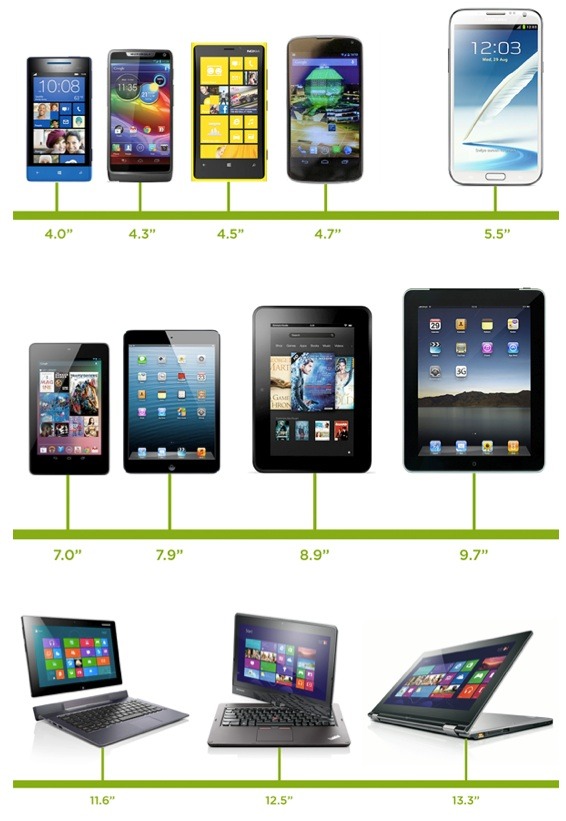
\includegraphics[width=0.75\textwidth]{img/tnav-devices.jpg}
	\caption[Porovnanie zariadení vzhľadom na veľkosť displeja]{
		Porovnanie zariadení vzhľadom na veľkosť displeja \cite{navigation}.\\
		Prevzaté z http://www.lukew.com/ff/entry.asp?1649}
	\label{fig: tnavmobile}
\end{figure}

Keďže sa začínajú vyskytovať rovnaké rozlíšenia displaja na rozlične veľkých zariadeniach alebo opačne, je potrebné medzi zariadeniami rozlíšovať aj inými spôsobmi. Je potrebné správne poruzumieť jednotkám ,,pixel'' a ,,viewport''.

Na rozdiel od pixelu definovaného W3C pomocou pozorovacieho uhlu a vzdlialenosti \cite{w3cpixel} existujú rôzne iné bežne používané jednotky ,,CSS pixel'', ,,device pixel'' a ,,density-independent pixel'' \cite{pixelnotpixel}. CSS pixel je abstrakný, môže sa zvyšovať alebo zniživať, používa sa bežne v kóde na definovanie rozmerov elementov.  Device pixel je fyzický pixel nachádzajúci sa na zariadení. Pretože zariadenia majú stále viac fyzických pixelov a tým aj ich väčsiu hustotu, zaviedol sa pojem density-independent pixel. Ten je opäť abstraktný a predstavuje počet CSS pixelov optimálnych na prezeranie obsahu. Pokiaľ by nebol zavedený, tak zariadenia s veľkou hustotou pixelov by sa nedali použiť na bežné prezeranie obsahu, nakoľku pixely sú veľmi malé a zobrazený text alebo elementy by tak boli nečitaľné.

Viewport je celkové miesto potrebné na zobrazenie webovej stránky. Na mobilných zariadeniach je situácia komplikovanejšia, pretože stále existuje množstvo stránok, ktoré nie sú na ne optimalizované. Preto ho výrobcovia mobilných prehliadačov rozdelili na ,,layout viewport'' a ,,visual viewport''. \cite{pixelnotpixel} Layout viewport je pre rozmiestnenie elementov celej stránky a visual viewport je definovaný pre elemty po priblížení stránky tak, že sa nezmestila na displej zariadenia.

% subsubsection ve_kos_a_rozl_enie (end)

\subsubsection{Interakčné prostriedky} % (fold)
\label{ssub:interak_n_prostriedky}

Postupom času začína upadať používanie klasických stolových počítačov ovládaných pomocou klávesnice a myši a presadzujú sa nové druhy mobilných zariadení so vstupným interfejsom v podobe množstva senzorov, ale hlavne s dotykovou plochou. Tá sa ako ovládací prostriedok začína presadzovať okrem mobilných zariadení aj v notebookoch. Pri dizajne aplikácie je preto potrebné myslieť aj na takýchto používateľov. Okrem nich však existujú aj iné možnosti ovládania ako sú napríklad sledovanie pohybu pomocou web kamery, natočanie a posúvanie zariadenia získané pomocou gyroskupu a accelerometra či počúvanie hlasových povelov zaznamenaných cez mikrofón. Je tak potrebné brať do úvahy aj ďalšie možnosti.

% \newpage

\paragraph{Dotyk} % (fold)

Dôležitým prvkom v prípade mobilných zariadení je možnosť ovládania aplikácii jednou rukou. Mobilné zariadenia sú využívané takmer pri každej príležitesti či vo vonkajšom alebo vnútornom prostredí, preto je potrebné správne prispôsobiť vzhľad a rozmiestnenie ovládacích prvkov. Pre ne platí, že najjednoduchšie dosiahnuteľné časti sú v spodnej strane zariadenia a s postupom k hornému okraju možnosť dosiahnutia klesá \cite{mobilebooktouch}.

\begin{figure}[H]
        \centering
        \begin{subfigure}[b]{0.7\textwidth}
                \centering
                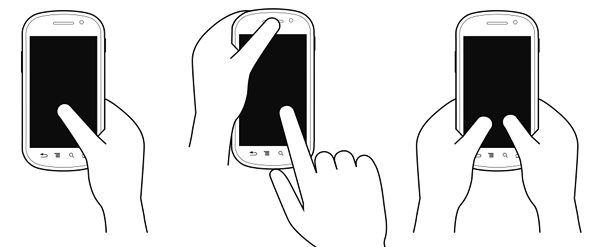
\includegraphics[width=\textwidth]{img/tnav-touch-phones.png}
        \end{subfigure}%
         %add desired spacing between images, e. g. ~, \quad, \qquad etc.
          %(or a blank line to force the subfigure onto a new line)
        \begin{subfigure}[b]{0.2\textwidth}
                \centering
                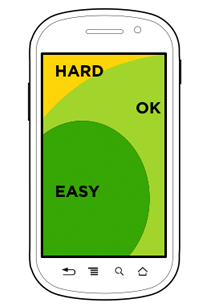
\includegraphics[width=\textwidth]{img/tnav-touch-phones2.png}
        \end{subfigure}

        \caption[Schopnosť ovládania mobilných telefónov]{Schopnosť ovládania mobilných telefónov \cite{navigation}.\\
		Prevzaté z http://www.lukew.com/ff/entry.asp?1649}
		\label{fig:tnavphones}
\end{figure}

Väčšie mobilné zariadenia alebo tablety už nie je možné pohodlne udržať v jednej ruke a tak je dôležité prispôsobiť ovládanie na dve ruky. Tablety sú držané v dvoch rukách za hranu a tak najlepšie dosiahnuteľné miesta sú na jeho okrajoch \cite{mobilebooktouch}.

\begin{figure}[H]
        \centering
        \begin{subfigure}[b]{0.6\textwidth}
                \centering
                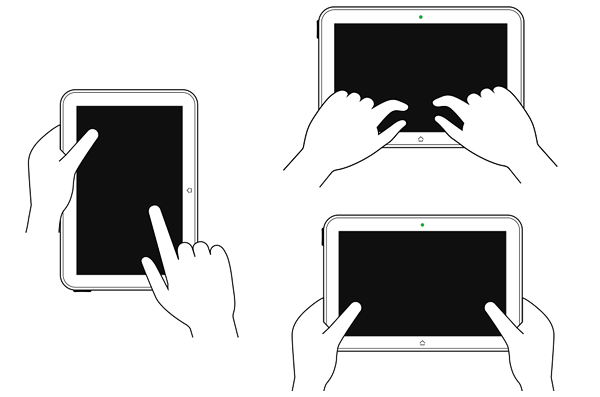
\includegraphics[width=\textwidth]{img/tnav-touch-tablets.png}
        \end{subfigure}%
         %add desired spacing between images, e. g. ~, \quad, \qquad etc.
          %(or a blank line to force the subfigure onto a new line)
        \begin{subfigure}[b]{0.4\textwidth}
                \centering
                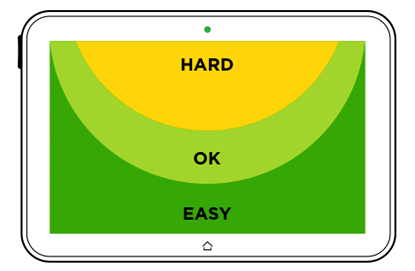
\includegraphics[width=\textwidth]{img/tnav-touch-tablets2.png}
        \end{subfigure}

        \caption[Schopnosť ovládania tabletov]{Schopnosť ovládania tabletov \cite{navigation}.\\
		Prevzaté z http://www.lukew.com/ff/entry.asp?1649}
		\label{fig:tnavtablets2}
\end{figure}

Podobné výsledky \cite{mobilebooktouch} sú aj pri novej kategórii zariadení, tzv. hybridných notebookov, ktoré okrem klávesnice obsahujú aj dotykový displej.

\begin{figure}[H]
	\centering
	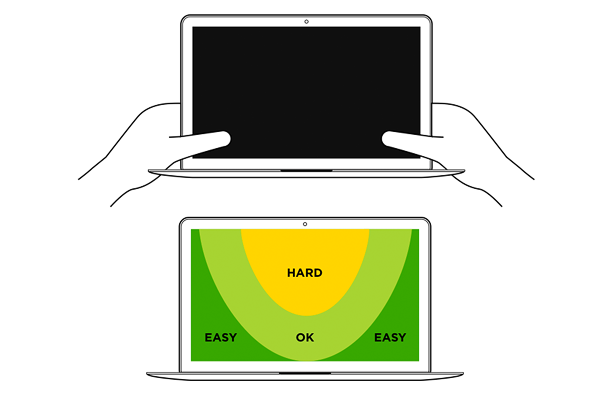
\includegraphics[width=0.6\textwidth]{img/tnav-touch-laptops.png}
	\caption[Schopnosť ovládania hybridných počítačov]{
		Schopnosť ovládania hybridných počítačov \cite{navigation}.\\
		Prevzaté z http://www.lukew.com/ff/entry.asp?1649}
	\label{fig: tnavlaptops}
\end{figure}



\paragraph{Reč} % (fold)

Možnosť rozpoznania reči vo webovej aplikácii je v súčasnosti experimentálna novinka a jej štandartizacia je zatiaľ veľmi ďaleko. Používateľ samozrejme musí explicitne povoliť použitie mikrofónu pre webovú aplikáciu. Špecifikácia je zatiaľ len vo forme návrhu a nie je ani zaradená do W3C štandartu HTML5 \cite{webspeechapi}. Podpora v prehliadočoch s enginom Blink sa však už nachádza od začiatku roku 2013 a základná funkčnosť bola odprezentovaná v rámci konferencie Google IO 2013. Rozpoznanie reči prebieha vzdialene na serveroch patriacich Googlu a zatiaľ neexistuje možnosť rozpoznania lokálne \cite{moreawesomeweb}.

S rozpoznaním reči je spojená aj jeho syntéza, alebo preklad textu na reč. Tá je na tom v súčasnosti čo sa týka podpory a implementácie v prehliadačoch ešte horšie. Experimentálna funkčnosť existuje len v posledných buildoch prehliadočov. Našťastie sa táto funkcionala dá čiastočne nahradiť volaniami vzdialených webových služieb ako je napríklad ,,Google Translate''. Takáto syntéza však už neprebieha na zariadení, ale len sa zo serveru príjme zvuková nahrávka, ktorá sa následne prehrá.

\paragraph{Kamera} % (fold)

Moderné webové prehliadače umožňujú získať prístup aj k video streamu z web kamery používateľa. Na prístup je rovnako potrebné povolenie od používateľa. Tento video stream prebieha vo zvolenej frekvencii a sa dá odchytiť a následne uložiť do elementu canvas, kde už sa k jednotlivým vzorkám pristupuje ako k obrázku. Je možné odfiltrovať okolie a zachovať len podstatné informácie na základe ktorých sa získa pohyb, respektíve gesto od používateľa.


\paragraph{Accelerometer a Gyroskop} % (fold)

Medzi dlhodobo podporované senzory najmä v mobilných zariadeniach patria accelerometer a gyroskop. Je k nim umožnený prístup priamo z webovej aplikácie aj bez priameho povolenia od používateľa.

Accelerometer slúží na získanie zrýchlenia zariadenia v osiach x, y a z, gyroskop na získanie uhlového zrýchlenia okolo týchto osí. Ich rozdiel je znázornený na nasledujúcom obrázku:

\begin{figure}[H]
  \centering
  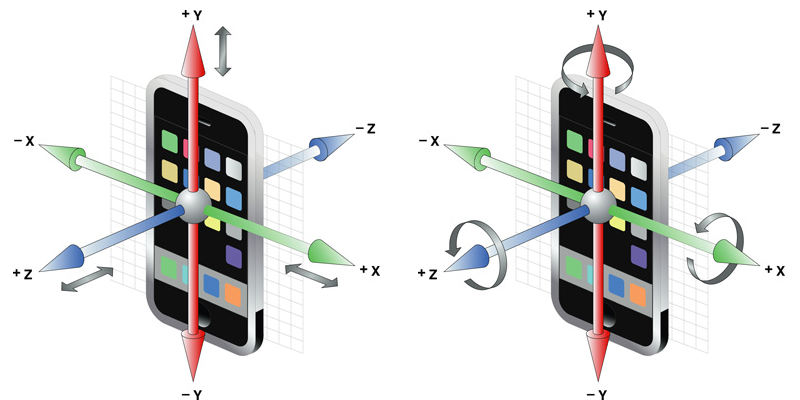
\includegraphics[width=0.8\textwidth]{img/accvsgyro.png}
  \caption[Accelerometor a gyroskop]{
    Zaznamenávané údaje pomocou accelerometora a gyroskopu}
  \label{fig: tnavlaptops}
\end{figure}

% subsubsection interak_n_prostriedky (end)


\subsubsection{Pripojenie} % (fold)
\label{ssub:pripojenie}

Spoločnou vlastnosťou webových aplikácii je, že pristupujú k rôznym zdrojom, ktoré sa môžu nachádzať okrem lokálneho úložiska aj na serverom, pomocou internetu. Spôsoby prenosu dát sú rôzne, od pevného pripojenie cez bezdrôtové až po mobilné, a každé z nich má iné vlastnosti.

V poslednom období sa spolu s mobilnými zariadeniami rozširuje aj používanie mobilného internetu. Keďže našim cieľom je, aby sa webová stránka načítala používateľovi čo najrýchlejšie, respektíve ak chceme aby sa používateľ na našu stránku prišiel a príchod si nerozmyslel pri jej dlhom načítavní, tak musíme šetriť množstvom prenášaných dát. Takéto šetrenie dát zároveň šetrí aj peňaženky používateľov \cite{performance}, hlavne pokiaľ sa jedná o roamingové dáta v zahraničí.

Načítanie webovej stránky sa skladá z viacerých fáz. Okrem samotnej konektivity používateľa aj spracovanie požiadavky serverom a následne vykonanie akcie v prehliadači. To je jediná fáza, ktorú môžeme ovplyvniť.

\begin{figure}[H]
	\centering
	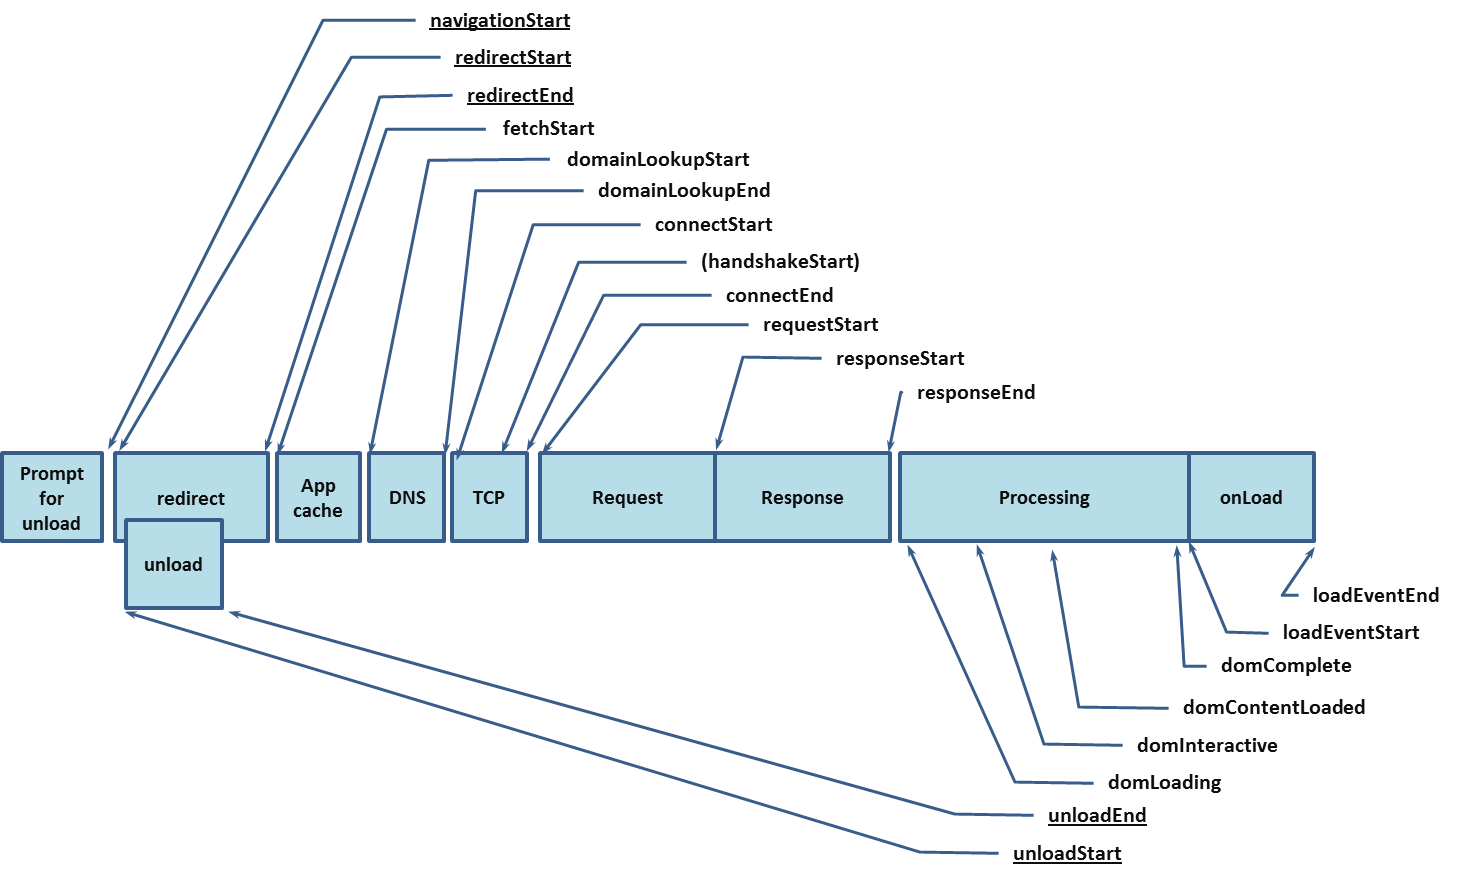
\includegraphics[width=1.0\textwidth]{img/w3c-timing-overview.png}
	\caption[Fázy spracovania požiadavky na server]{
		Fázy spracovania požiadavky na server \cite{timing}.\\
		Prevzaté z http://www.w3.org/TR/navigation-timing/}
	\label{fig: timing}
\end{figure}

Tieto fázy môžme aj priamo merať pomocou interfacu \url{performance.timing}, ktorý ich zobrazuje priamo v podobe času \cite{1000ms, performancebrowsernetworking}. Vďaka tomu máme dokonalejší prehľad o používateľovom pripojení a vieme mu tak prispôsobiť jednotlivé komponenty stránky. W3C špecifikácia je vo fáze ,,Recommendation'' \cite{timing}, ale stále hlavnou nevýhodou je chýbajúca podpora v niektorých prehliadačoch. Čiastočnou náhradou je meranie rozdielov dvoch časov, ale tak získame dáta len zo spracovania požiadavky na strane klienta.

\begin{figure}[H]
	\centering
	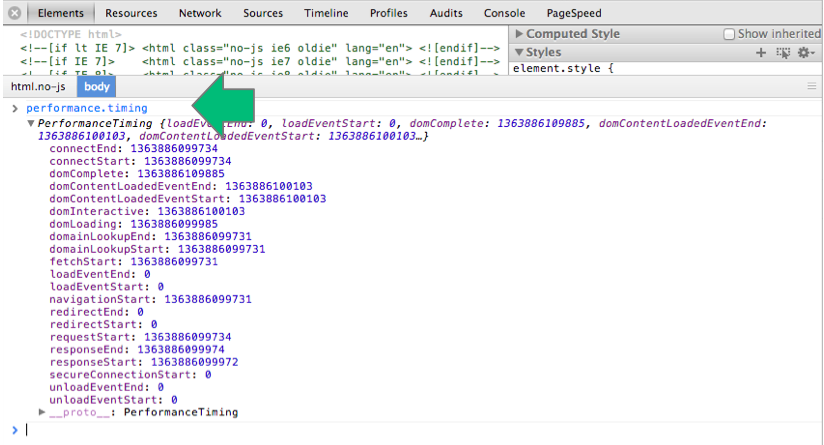
\includegraphics[width=1.0\textwidth]{img/1000ms.png}
	\caption[Čas potrebný na spracovanie požiadavky na server]{
		Čas potrebný na spracovanie požiadavky na server.}
	\label{fig: 1000ms}
\end{figure}

Každá požiadavka na server niečo stojí. Ideálny prípad je taký, že medzi zariadením a serverom sa neprenášajú žiadne dáta a všetky prístupy ku zdrojom sa riešia len z lokálneho úložiska. V prípade internetových aplikácii to však väčšinou nie je úplne možné, pretože používateľ chce pristupovať k čo najčerstvejším dátam. Cieľom je však čo najviac limitovať požiadavky na server.

To, či je vôbec používateľ pripojený na internet vieme zistiť pomocou interfacu \url{navigator.onLine}, ktorý vráti hodnotu ,,true'' alebo ,,false'' a takisto môžme počúvať na zmeny pripojenia vďaka ,,event listenerom'' na \url{window.online} a \url{window.offline}.

Rýchlosť, akou je používateľ pripojený na internet, je dostupná v objekte \url{navigator.connection} pod atribútom ,,bandwidth'' charakterizujúcej pripojenie v MB/s \cite{network}. V prípade zmeny rýchlosti je rovnako vyvolaný ,,event''. Nevýhodou je zatiaľ slabá podpora zo strany prehliadačov.

% subsubsection pripojenie (end)

\newpage
\subsubsection{Platforma} % (fold)
\label{ssub:platforma}

Rozhodovanie sa na základe platformy je taktiež veľmi dôležité. Umožňuje nám jednak zjednošiť dizajn a zmenšiť počet potrebných komponentov na webovej stránke, ale taktiež vytvárať cielenú reklamu. Rozlišovanie prebieha na základe pola ,,user agent'' špecifickom pre každý prehliadač, respektíve operačný systém.

V prípade zisťovania podpory jednotlivých vlastností je však lepšie priamo zisťovať podporu komponentu zo strany prehliadača ako zisťovaním a porovnaním s platformou. Nemusíme si tak udržiavať databázu a neustále ju aktualizovať. Takéto riešenie je preto z pohľadu vývoja lepšie pre budúcnosť.

% subsubsection platforma (end)

% subsection mo_nosti_prisp_sobenia (end)


\subsection{Adaptačné techniky \footnote{Tejto kapitole som sa už z časti venoval vo svojej bakalárskej práci Tvorba bohatých internetových aplikácií pre mobilné zariadenia \cite{ja}. V tomto dokumente sa nachádza rozšírená verzia doplnená o novo vzniknuté techniky adaptácie.}} % (fold)
\label{sub:adapta_n_techniky}

S príchodom prvých mobilných zariadení existoval rozdiel medzi mobilným webom a webom pre desktopy a tak bolo pomocou servera jednoduché zistiť, aká verzia sa má zariadeniu zobraziť.

Pretože dnes už existuje mnoho zariadení od mobilných cez tablety až po klasické počítače a vzájomne sa prelínajú, je potrebné zabezpečiť, aby sa webový obsah zobrazoval správne na každom z nich.

\begin{fancybox}
\textit{,,There is no Mobile Web. There is only The Web, which we view in different ways. There is also no Desktop Web. Or Tablet Web. Thank you.'' Stephen Hay} \cite{noMobileWeb}
\end{fancybox}

Tento výrok bol vyslovený už pred niekoľkými rokmi a v súčasnosti pri prelínaní rôznych zariadení sa stále viac potvrdzuje. Pre vývoj webovej stránky alebo aplikácie existuje viacero spôsobov \cite{mobiforge}, každý má svoje výhody a nevýhody. Správnosť výberu konkrétnej metódy záleži od toho, či ideme upravovať už existujúcu webovú verziu na rôzne zariadenia alebo či vytvárame novú aplikáciu a v neposlednom rade aj od vynaloženého úsilia či financií.


\subsubsection{Responsive design} % (fold)
\label{ssub:responsive_design}

Pojem ,,Responsive design'' bol pôvodne súbor pravidiel tvorby dizajnu pre rôzne rozlíšenia, ktoré definoval Ethan Marcotte v článku Responsive design v roku 2010. Všetkým zariadeniam je posielaný rovnaký HTML a javascript, rozdiel je len v designe. Design sa zakladá na používaní flexibelného vzhľadu stránky, ktorý sa prispôsoboval rôznym zariadeniam, flexibilných obrázkoch, ktoré sa prispôsobujú vzhľadu a CSS media queries. \cite{responsive, mediaqueries} Až neskôr bol označený ako metóda na dosiahnutie výsledku.

Tvorba vzhľadu pomocou Responsive design znamená používanie hodnôt v percentuálnom pomere namiesto statických hodnôt, obrázky sú prepojené s elementom stránky, majú nastavené jeho plné rozmery a automaticky sa prispôsobujú jeho zmenám. Vytvára sa stránka pre väčšie rozlíšenie a pomocou CSS media queries sa môžu aplikovať rôzne pravidlá pre jednotlivé elementy na základe rozlíšenia zariadenia, jeho orientácie či pomeru strán. Pri použití takéhoto prístupu však nastávajú problémy na mobilných zariadeniach s menším rozlíšením displeja a na väčších zariadeniach ako sú televízory.\\


% \begin{center}
% 	\includegraphics[width=1.00\textwidth]{img/responsive.png}
% 	\captionof{figure}{Stránka http://www.londonandpartners.com/ na rôznych zariadeniach}
% 	\label{fig: responsiveImg}
% \end{center}

\paragraph{Výhody:}
\begin{itemize}
	\item dobrá metóda na dosiahnutie nezávislosti zobrazenia obsahu pri rôznom rozlíšení zariadení, stránka vyzerá inak v mobilnom zariadení ako v tablete alebo stolnom počítači
	\item rýchly vývoj aplikácie
\end{itemize}

\paragraph{Nevýhody:}
\begin{itemize}
	\item neumožňuje prispôsebenie obsahu, ale len jeho vzhľad
	\item mobilné zariadenie sťahuje plnú veľkosť obrázka, ale vidí ho v menšom rozlíšení
	\item problémy pri zariadeniach s nižším a väčším rozlíšením
\end{itemize}

% subsubsection responsive_design (end)


\subsubsection{Mobile First} % (fold)
\label{ssub:mobile_first_responsive_design}

Problémy pri správnom zobrazení stránky na zariadeniach s nižším rozlíšením podnietili vznik novej metódy dizajnu - ,,Mobile First''. Základ tvorí metóda Responsive design, ale pôvodný návrh stránky sa nerobí pre desktopovú verziu ale na malé rozlíšenie. Až pomocou media queries sa pridávajú elementy pre väčšie rozlíšenie. Takto sa pokryju všetky zariadenia od najmänších po najväčšie a webová stránka je pripravená na zariadenia, ktoré vzniknú aj v budúcnosti.

Technika Mobile First však okrem samotného dizajnu zahŕňa aj optimalizáciu webu pre používateľa či už z pohľadu UX alebo výkonu \cite{mobilefirst}.

\paragraph{Výhody:}
\begin{itemize}
	\item dosiahnutie nezávislosti zobrazenia obsahu pri rôznom rozlíšení zariadení
	\item podporuje všetky zariadenia od najmenších po najväčšie, stránka je pripravená aj na ,,zariadenia budúcnosti''
\end{itemize}

\paragraph{Nevýhody:}
\begin{itemize}
	\item stále neumožňuje prispôsebenie obsahu, ale len jeho vzhľad
	\item dizajn stránky musí byť vytvorený od základu, čo však môže byť aj východa
\end{itemize}

% subsubsection mobile_first_responsive_design (end)

\subsubsection{Progressive enhancement} % (fold)
\label{ssub:progressive_enhancement}

V poslednom období sa stáva veľmi popolárnou metódou Progressive Enhancement. Táto metóda je založená na princípe posielania rovnakého html, javascriptu a iných zdrojových súborov všetkým zariadeniam. Následné vykonávanie aplikácie sa presúva zo strany servera a prebieha na klientovi pomocou javascriptu, kde je už možné presne špecifikovať, čo sa má kedy a ako vykonávať. Používateľovi sa sprístupňujú pokročilejšie vlastností aplikácie len ak ich podporuje používaný webový prehliadač, respektíve zariadenie. Taktiež je možné načítavať objekty zo servera len vtedy, keď sú potrebné, a tým sa zabraňuje zbytočným prenosom dát. Pri spojení tejto metódy s HTML5 je dokonca možné tvoriť offline klientské aplikácie.

Pokiaľ chceme pokryť celé spektrum zariadení tak je implementácia pomocou tejto metódy náročnejšia. V spojení s metódou reseponsive design je to najlepšie možné riešenie na prispôsobenie si obsahu a vzhľadu aplikácie.

\paragraph{Výhody:}
\begin{itemize}
	\item úplne prispôsobenie obsahu a vzhľadu, minimálne alebo žiadne dátove prenosy
\end{itemize}

\paragraph{Nevýhody:}
\begin{itemize}
	\item náročnejšia implementácia, 
	\item rýchlosť vykonávania aplikácie závisi od výkonu zariadenia
\end{itemize}

% subsubsection progressive_enhancement (end)

\subsubsection{Graceful degradation} % (fold)
\label{ssub:graceful_degradation}

Opak metódy Progressive enhancement sa nazýva Graceful degradation. Používateľovi sa predáva plne funkčná aplikácia nadizajnovaná na najlepšie zariadenia, kde sa na jednotlivé pokročilejšie funkcie postupne vypínajú vzhľadom na použité zariadenie. Používa sa často na upravenie súčasnej nasadenej verzie na potreby mobilných zariadení.

\begin{figure}[H]
	\centering
	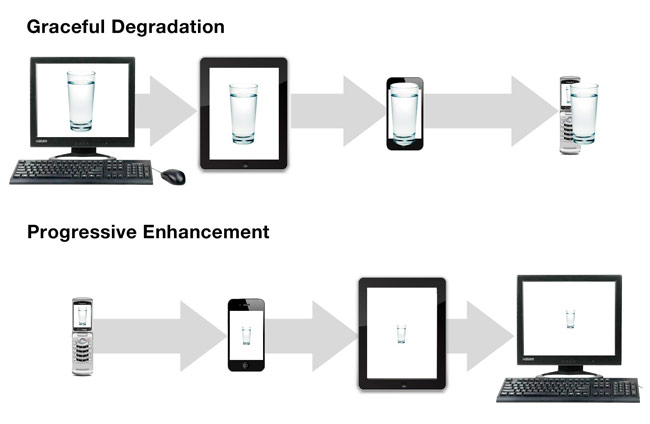
\includegraphics[width=0.8\textwidth]{img/PEvsGD.jpg}
	\caption[Progressive enhancement vs Graceful degradation]{
		Progressive enhancement vs Graceful degradation \cite{adaptivesxsw}.\\
		Prevzaté z http://bradfrostweb.com/blog/web/mobile-first-responsive-web-design/}
	\label{fig: gd}
\end{figure}

\paragraph{Výhody:}
\begin{itemize}
	\item prispôsobenie obsahu a vzhľadu na jednoducšie zariadenia
	\item zachovanie súčasnej verzie webovej stránky
\end{itemize}

\paragraph{Nevýhody:}
\begin{itemize}
	\item nezohľadňuje budúce zariadenia, už v súčasnosti majú niektoré tablety kvalitnejšie displeje ako stolové počítače 
\end{itemize}

% subsubsection graceful_degradation (end)


\subsubsection{Server-side Adaptation} % (fold)
\label{ssub:ress_}

Metóda Server-side Adaptation je používaná väčšinou webových stránok na detekovanie mobilného zariadenia a v súčasnosti patrí už medzi historické techniky. Pri prístupe na stránku sa pomocou servera detekuje zariadenie a je mu ponuknutá vhodná verzia stránky, väčšinou dochádza k presmerovaniu (na mobilnú verziu). Celá logika aplikácie sa nachádza na serveri. Stránka môže byť presne vytvorená pre dané zariadenie, takže nenastávajú problémy pri dizajne, je však potrebné mať na serveri nainštalovanú knižnicu na jeho detekovanie\footnote{napríklad DeviceAtlas alebo WURFL založené na detekovaní pola user agent}. Detekcia zariadenia je pri priamej návšteve stránky cez prehliadač úspešná, k problémom však prichádza pri návšteve stránky cez iných klientov. Taktiež je dôležité mať databázu zariadení neustále aktualizovanú.

\paragraph{Výhody:}
\begin{itemize}
	\item zobrazenie vhodnej stránky pre zariadenie, nesťahuje sa nepotrebný obsah
\end{itemize}

\paragraph{Nevýhody:}
\begin{itemize}
	\item potreba knižníc na detekovanie zariadenia, ktorú je nutnú neustále aktualizovať
	\item dlhšie načítavanie stránky na pomalšom internetovom pripojení, pretože dochádza k presmerovaniu
\end{itemize}

% subsubsection ress_ (end)

\subsubsection{RESS (Responsive Design + Server Side Components)} % (fold)
\label{ssub:ress_responsive_design_server_side_components_}

Kombináciou techník Responsive Design a Server-side Adaptation vznikla novšia technika adaptácie. Pre každé zariadenie sa na serveri dynamicky vygenerujú pre neho špecifické časti webovej aplikácie, ktoré sa mu následne zobrazia a upravia pomocou responsive dizajnu.

\paragraph{Výhody:}
\begin{itemize}
	\item jednoduchšia udržiaveteľnosť, neexistujú rôzne verzie stránky ale len jedna
\end{itemize}

\paragraph{Nevýhody:}
\begin{itemize}
	\item potreba nainštalovaných knižníc na detekovanie zariadenia
	\item náročnejšia implementácia na strane servera
\end{itemize}

% subsubsection ress_responsive_design_server_side_components_ (end)

% subsection adapt_cia (end)

\newpage
\section{Nástroj na overenie} % (fold)
\label{sec:n_stroj_na_overenie}
Ako nástroj na overenie sa vytvorila knižnica s názvom Angular-Adaptive \footnote{Angular-Adaptive \url{http://angular-adaptive.github.io/} je sprievodca vo svete adaptívneho web dizajnu.} do populárneho JavaScriptového frameworku AngularJS \footnote{AngularJS \url{http://angularjs.org/} je populárny JavaScriptový framework, ktorý rozširuje HTML o nové možnosti pre webové aplikácie.}, kde sa následne skúmali možnosti adaptácie komponentov. Hlavným dôvodom výberu AngularJS bola možnosť vytvárania modulov, ktoré sa dajú následne jednoducho použivať vo webových projektoch. Takáto podpora vytvárania externých modulov bude už o pár rokov natívna v prehliadačoch vďaka webovým komponentom \cite{webcomponents}. Samotná distribúcia modulov prebieha pomocou balíčkovaciemu nástroja Bower \footnote{Bower \url{http://bower.io/} je balíčkovací manažér pre web.}.

\subsection{Alternatívne spôsoby ovládania} % (fold)
\label{sub:alternat_vne_sp_soby_ovl_dania}

\subsubsection{Reč} % (fold)
\label{ssub:re_}

% subsubsection re_ (end)


\subsubsection{Pohyb} % (fold)
\label{ssub:pohyb}

\begin{figure}[H]
  \centering
  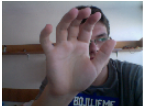
\includegraphics[width=0.3\textwidth]{img/motion/video.png}
  \caption[Pohyb - video]{
    Pohyb - video}
  \label{fig: motion-video}
\end{figure}

\begin{figure}[H]
  \centering
  
\includegraphics[width=0.3\textwidth]{img/motion/skin.png}
  \caption[Pohyb - detekcia kože]{
    Pohyb - detekcia kože}
  \label{fig: motion-skin}
\end{figure}

\begin{figure}[H]
  \centering
  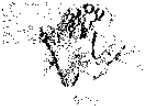
\includegraphics[width=0.3\textwidth]{img/motion/edges.png}
  \caption[Pohyb - detekcia hrán]{
    Pohyb - detekcia hrán}
  \label{fig: motion-edges}
\end{figure}

% subsubsection pohyb (end)

\subsubsection{Gyroskop} % (fold)
\label{ssub:gyroskop}


The specs suggest the following:

\begin{itemize}
  \item X is in the plane of the ground and is positive to the East (-ive to West)
  \item Y is in the plane of the ground and is positive to the North (-ive to South)
  \item Z is perpendicular to the ground plane and is positive towards the sky (negative into the earth)
\end{itemize}

Rotation should be expressed using the right hand rule, thus positive values with rotation clockwise around the axis of rotation when looking down the axis.

The tables below express where the zero point is for a given axis, what the values are for it's rotational range, whether it obeys the Right Hand Rule* and any further notes.

RHR* = Right Hand Rule. That positive values increase when rotating clockwise
around the axis of rotation when looking along the axis' postive trajectory. This causes confusion because for a compass it looks like you're going backwards but that's because you're looking along the -ive trajectory of the Z axis.

Alpha:

The spec is unclear what the defaults should be and so as a result many different choices are taken by the vendors. This causes confusion and the spec is not clear about what 0 degrees should actually be. From the example it is implied that North is 0 degrees because West is given as +90 degrees (which is correct under the RHR).

The range is tested by holding the device level in the horizontal plane, orienting it to the zero point then turning it through 360 degrees, observing its range and direction

\begin{table}[H]
  \begin{tabular}{ | l | l | l | l |}
  \hline
              & Zero point  & RHR   & Range \\ \hline
  Reference   & North (0)   & Y     & [0, 360] \\  
  iOS Chome   & East (90)   & Y     & [0, 360] \\  
  iOS Safari  & East (90)   & Y     & [0, 360] \\  
  Android & & & \\  
  Chrome      & North (0)   & Y     & [0, 360] \\  
  Stock       & West (270)  & Y     & [0, 360] \\  
  Firefox     & North (0)   & N     & [0, 360] \\
  \hline
  \end{tabular}
  \caption[Alpha rotácia gyroskopu]{Alpha rotácia gyroskopu}
\end{table}

Beta:

The spec defines zero point as being flat in the horizontal plane. All browsers now support this model. Note that there are some issues in the ranging of the values.

The range is tested by holding the device level in the horizontal plan and confirming the zero point. The device is then rotated around the X axis through 90 degrees (screen faces observer), then through the next 90 degrees (screen face down), then the remaining 180 degrees completing the bottom portion of the rotation.

\begin{table}[H]
  \begin{tabular}{ | l | l | l | l | l |}
  \hline
              & Zero point    & RHR   & Range         & Notes\\ \hline
  Reference   & Horiz Plane   & Y     & [0, -180|180] & \\  
  iOS Chome   & Horiz Plane   & Y     & [-90, 90]     & Full range of rotation not supported. \\  
  iOS Safari  & Horiz Plane   & Y     & [-90, 90]     & Full range of rotation not supported. \\  
  Android & & & & \\  
  Chrome      & Horiz Plane   & Y     & [-90, 90]     & Full range of rotation not supported. \\  
  Stock       & Horiz Plane   & Y     & [-90, 90]     & Full range of rotation not supported. \\  
  Firefox     & Horiz Plane   & N     & [0, 180|-180] & Back to front \\
  \hline
  \end{tabular}
  \caption[Beta rotácia gyroskopu]{Beta rotácia gyroskopu}
\end{table}

Under iOS as well as the stock Android browser and Chrome for Android, the rotation goes the right direction from the horizontal plane however once it hits the maximal or minimal point at (90 | -90 degrees) it simply starts to decrease again, rather than provide the full rotation.

In FF on android the rotation is back to front but it does go through the full range to 180 degrees. However under firefox the value is -90 when the top is point upwards and 90 when the top of the device points downwards. This is a reversing of the RHR.

Gamma:

The spec defines the zero point as being level in the horizontal place. Again there are some issues with ranges and some implied issues with how the W3C have defined this as they are assuming only 90 degrees of rotation around the Y axis is relevant.

The range is tested by holding the device level in the horizontal plane and confirming a zero point. The device it then rotated around the Y axis 90 degrees clockwise (screen faces right) then again (screen faces down) and then through the other 180 degrees back to the origin.

\begin{table}[H]
  \begin{tabular}{ | l | l | l | l | l |}
  \hline
              & Zero point    & RHR   & Range         & Notes\\ \hline
  Reference   & Horiz Plane   & Y     & [0, 90|-90]   & Poor definition by the W3C \\  
  iOS Chome   & Horiz Plane   & Y     & [0, 180|-180] & Full range of rotation not supported \\  
  iOS Safari  & Horiz Plane   & Y     & [0, 180|-180] & Full range of rotation not supported. \\  
  Android & & & & \\  
  Chrome      & Horiz Plane   & Y     & [0, 270|-90]  & Odd range to cope with the gaps \\  
  Stock       & Horiz Plane   & Y     & [0, 270|-90]  & Odd range to cope with the gaps \\  
  Firefox     & Horiz Plane   & N     & [0, -90|90]   & Range back to front \\
  \hline
  \end{tabular}
  \caption[Gamma rotácia gyroskopu]{Gamma rotácia gyroskopu}
\end{table}

This is poor definition by the W3C as it implies rotation only happens to 90 degrees from the horizontal plane, thus causing an issue when you go under this.

Under iOS rotation starts from the horizontal plan with the screen facing up as the zero point. Rotating around the Y axis so that the screen is facing down will result in a value of 180 or -180. If the rotation occurs clockwise the values increase through the +ive range, if the rotation is anti-clockwise then the values increase through the -ive range. Thus resting the R edge (L edge upwards) the value is 90, the reverse (resting on the L edge, R edge up) means the value is -90.

The Chrome for Android and stock android browsers create the right rotational vales for the +-90 range however the gap after 90 on the clockwise rotation is filled with increasing +ive values until it reaches the -90 value. This provides an opportunity to know exactly how far the device is rotated around the Y axis but can't be replicated by any of the others.

Firefox reverses its range the same way as it does on Beta. The range is correct however rotation clockwise results in a -ive number and the reverse.



\paragraph{Gyrocopter} % (fold)
\label{par:gyrocopter}

\begin{figure}[H]
  \centering
  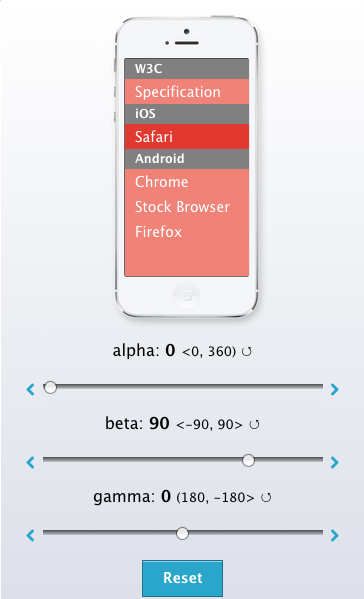
\includegraphics[width=0.5\textwidth]{img/gyrocopter.png}
  \caption[Gyrocopter - gyroskop simulátor]{
    Gyrocopter - gyroskop simulátor}
  \label{fig: gyrocopter}
\end{figure}

% paragraph gyrocopter (end)

% subsubsection gyroskop (end)

% subsection alternat_vne_sp_soby_ovl_dania (end)

\subsection{Komponenty} % (fold)
\label{sub:komponenty}

\subsubsection{Video} % (fold)
\label{subsub:video}

Populárnym doplnkom súčasných webový stránok je priložené video, ktoré sa často nachádza na serveroch YouTube alebo Vimeo.

Problémom je, že pri vložení videa pomocou iframe alebo embed api sa uskotočňuje množstvo dopytov na servery a prenášajú sa zbytočné dáta aj keď používateľa video nezaujíma a vôbec si ho neprehrá. Okrem zbytočne prenášaných dát sa aj znižuje výkon, nakoľko určitý čas trvá spracovanie požiadaviek.

Nasledujúce dáta sa prenesú pri zobrazení stránky, na ktorú bolo vložené video zo servera YouTube pomocou dostupného iframe API:

\begin{figure}[H]
	\centering
	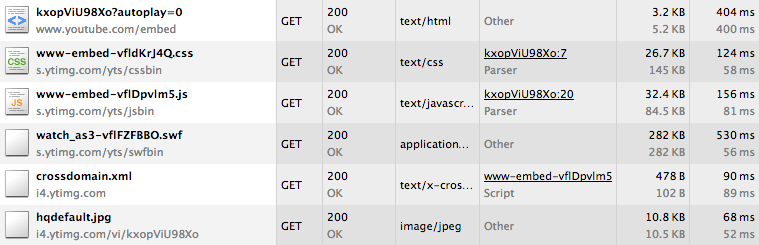
\includegraphics[width=1.0\textwidth]{img/youtube.png}
	\caption[Prenášané dáta pri požiadavke na video zo servera YouTube]{
		Prenášané dáta pri požiadavke na video zo servera YouTube}
	\label{fig: youtube}
\end{figure}

Celkovo sa vykoná 6 požiadaviek a prenesie sa 350 kB dát bez toho, aby používateľ spustil video. Podobná situácia sa opakuje aj pri požiadavke na video zo servera Vimeo pomocou iframe API.

\newpage
\begin{figure}[H]
	\centering
	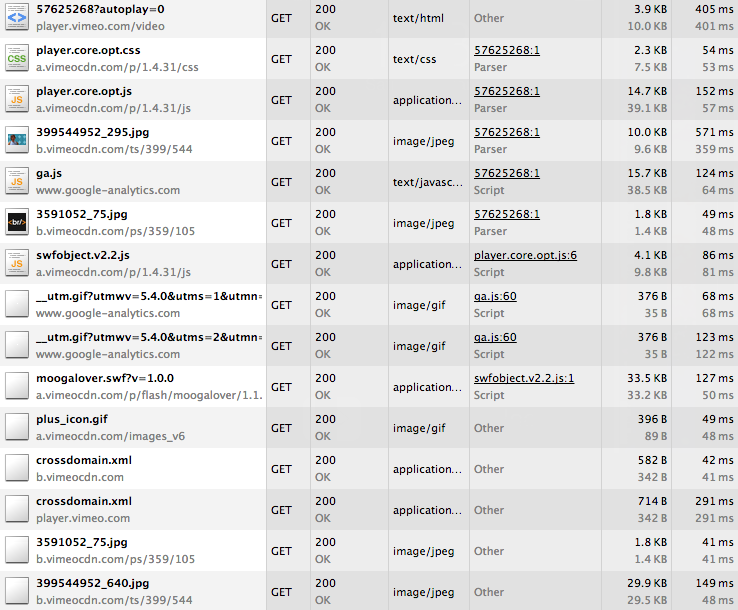
\includegraphics[width=1.0\textwidth]{img/vimeo.png}
	\caption[Prenášané dáta pri požiadavke na video zo servera Vimeo]{
		Prenášané dáta pri požiadavke na video zo servera Vimeo}
	\label{fig: vimeo}
\end{figure}

V tomto prípade sa dokonca vykoná 15 požiadaviek a prenesie sa 120 kB dát. V prípade použitia javascriptového API s HTML 5 prehrávačom videa sa síce nestiahnú flashové komponenty, ale nahradia ich rovnakoveľké javascriptové súbory.

Lepšie riešenie je použiť podmienené načítavanie. Najskôr sa načíta len obrázok videa a pridajú sa jednoduché štylistické prvky aby vytvorený element pripomínal video súbor a až po kliknutí sa urobia dopyty na vzdialený server s automatickým prehratím videa. Výhodou takéhoto riešenia je zmenšenie veľkosti dopytov a s tým spojené šetrenie dát používateľov. 

Čo sa týka získania obrázkového náhľadu videa, tak YouTube túto možnosť priamo poskytuje a záleží len od identifikátora videa. K obrázku je tak možné pristúpiť priamo. Navyše po vykonaní požiadaviek na server po kliknutí na obrázok a následnom spustení videa pomocou api sa už daný onrázok nachádza v pamäti, tak sa nemusia robiť ďalšie požiadavky. 

Samotný proces automatického spustenia YouTube videa nie je úplne jednoduchý, nakoľko nastavenie hodnoty ,,autoplay'' pri vložení elementu iframe s videom na stránku nefunguje na mobilnom prehliadači Safari, kde je táto možnosť zakázaná. V takomto prípade by sa po kliknutí na obrázok videa načítal len element s videom a aby sa samotné video začalo prehrávať očakáva sa ďalšie kliknutie. Takéto správanie je neželené a je proti používateľskému zážitku. 

Preto bolo potrebné vymyslieť lepšie riešenie. To spočíva v načítaní scriptu s javascriptovým youtube API a následným vytvorením iframe elementu s videom až pomocou neho. Takto máme prístup k programátorskému ovládaniu prehravača videa a môžme ho spustiť keď potrebujeme, teda po kliknutí na obrázok s náhľadom videa. Takéto riešenie už fungujé aj na iOS s mobilným prehliadačom Safari.

Stále však máme problém pri staršej verzii iOS 5 a menej, tam nefunguje ani programátorske spustenie videa. V tejto verzii iOS sa však ešte distribuovala predinštalovaná aplikácia na prehrávanie Youtube videí, ktorá bola v neskorších verziách odstránená a je ju možné stiahnúť z iTunes. Výhodou je, že video môžme otvoriť priamo v nej pomocou youtube url schémy. Musíme však používaný prehliadač správne detekovať a následne sa rozhodnúť, aké prehrávanie zvolíme.

Na detekovanie funkcionality otvorenia youtube videa v aplikácii pomocou systému iOS a jej zisťovaním len z pola ,,user agent'' nie je správne, nakoľko by bolo potrebné získať úplne všetky verzie systému, ktorých je mnoho, a následne porovnať s verziou zariadenia.

Lepším riešením je vytvorenie testu funkčnosti prehrávania videa, ktoré je riešené pomocou nástroja Modernizr\footnote{Modernizr \url{http://modernizr.com/} je JavaScriptová knižnica, ktorá detekuje dostupnosť natívnej imlementácie nových technológií v prehliadači.} umožňujúcim detekciu základných HTML5 a CSS3 vlastností prehliadača a vytváranie vlastných testov. Následne sa na základe výsledku testu rozhodnemu akú akciu vykonať. Problémom je, že testy sa vykonávajú po načítaní stránky a nechceme používateľovi automaticky otvoriť natívnu aplikáciu alebo ho presmerovať na stránky youtube. Preto je zvolená iná varianta a detekuje sa podbora vlastnosti, ktorá bola pridaná až v novšej verzii iOS 6. Konkrétne sa jedná o podboru jednotiek ,,vh a vw'' (viewport height a viewport width) slúžiacich na nastavenie veľkosti DOM elementu. Detekcia či je zariadenie iOS vychádza z pola user agent, ale už sa nezisťuje jej verzia.

Výsledok je taký, že po kliknutí na obrázok s náhľadom videa a vyhodnotení testu prehrávania sa začne prehrávať v prehliadači alebo v natívnej aplikácii.

V prípade Vimea je situácia trochu komplikovanejšia pretože k náhľadovému obrázku sa priamo nevieme dostať a je potrebné urobiť jednu požiadavku na API, ktorá vráti informácie o videu. Vykonanie požiadavky síca nejaký čas trvá, ale aj tak je výsledok z pohľadu prenášaný údajov lepší ako robiť požiadavku priamo na samotné video.

S prehrávaním videa zo služby vimeo je situácia podobná, neexistuje však natívna aplikácia a po klinutí na náhľad videa je používateľ v starších verziách iOS presmerovaný na stránky vimea, v novších verziách iOS a v Androide sa mu automaticky prehrá.

% subsubsection video (end)


\subsubsection{Mapy} % (fold)
\label{subsub:mapy}

Mapy podobne ako videá vytvárajú nechcené dátové prenosy, dokonca ich ešte aj prevyšujú pretože sa neprenášajú len údaje o aktuálne zobrazenej časti mapy ale aj jej okolie. Okrem nich navyše na webe neposkytujú taký plnohodnotný zážitok z prezerania ako v natívnej aplikácii. Nevýhodou je aj nemožnosť posúvania webovej stránky pokiaľ je element s mapou väčší ako je rozlíšenie displeja mobilného zariadenia, lebo eventy sú zachytávané mapou a posúva sa tá.

Používateľ nemusí chcieť okamžite interagovať s mapou a v takomto prípade ho zbytočne zaťažuje. Výhodnejšie je tak zobraziť len náhľad mapy, ktorý sa načíta rýchlejšie pretože šetrí prenášané dáta, a pokiaľ sa používateľ chce dozvedieť viac, tak len jednoducho na mapu klikne. V takomto prípade sa mu automaticky načíta plne interaktívna mapa. Na zobrazenie náhľadu mapy existuje API v službe google maps\footnote{\url{https://developers.google.com/maps/documentation/staticmaps/}}, takže je možné využiť priamo to. Nevýhodou je, že počet požiadaviek za deň, ktoré sú zadarmo, je obmedzený, po získaní API kľúča je možné ich spraviť 25000, ďalšie sú spoplatňované.

Rozšírením na mobilných zariadeniach iOS je možnosť otvorenia mapy priamo v natívnej aplikácii, ktorá prináša ešte väčší používateľský zážitok ako zobrazenie na webe. To je uskutočňované pomocou url schémy. V starších verziách iOS sa nachádzala natívna aplikácia na Google API a bola vyvolaná otvorením nasledujúceho odkazu, kde bolo možné zadávať parametre zobrazenia.

\begin{verbatim}
http://maps.google.com/
\end{verbatim}

S príchodom iOS 6 bola aplikácia nahradená vlastnom Apple aplikáciou, na ktorej spustenie sa zmenila aj url schéma a pôvodná otvorí mapu len v prehliadači. Výhodou je, že na starších, respektíve nepodporovaných zariadeniach nastáva presmerovanie na stránky Google a tak na rovnakom odkaze funguje spúšťanie aj pôvodnej aplikácie. Nová url schéma má nasledujúci tvar:

\begin{verbatim}
http://maps.apple.com/
\end{verbatim}

% subsubsection mapy (end)


\subsubsection{Lightboxy} % (fold)
\label{subsub:lightboxy}

Lightbox je technika umožňujúca zobrazovať webový obsah v modálnych oknách nachádzajúcich sa nad úrovňou pôvodnej stránky.

Hlavným problémom použitia ,,lightboxov'' na mobilných zariadeniach je nesprávne zobrazovanie stránok pokiaľ nové okno je väčšie ako displej. V takomto prípade by bolo vhodnejšie používateľa presmerovať priamo na novú stránku.

% subsubsection lightboxy (end)

\subsubsection{Otvorenie v aplikácii / Stiahnutie aplikácie} % (fold)
\label{ssub:otvorenie_v_aplik_cii}

V súčasnosti sme opklopovaný množstvom informačných zdrojov, ktoré sa zväčša nachádzajú na internete dostupné na konkrétnej webovej adrese. Na tieto zdroje existuje množstvo odkazov z rôznych webových stránok, sociálnych sietí či mobilných aplikácii, ktoré zobrazia ich obsah v prehliadači.

\begin{fancybox}
\textit{,,Links don’t open apps.'' Jason Grigsby} \cite{links}
\end{fancybox}

Webové odkazy neotvárajú natívne aplikácie, čo je technicky pravda, no realita je trochu odlišná. Prepojenie webovej časti aplikácie s natívnou umožňuje otvárať komplexnejšie úlohy, na ktoré je vo webe nedostatočny výkon, priamo v natívnom kóde. To umožní plynulejší chod aplikácie a lepší používateľský zážitok.

Prepájanie aplikácii sa uskutočňuje pomocou ,,custom url schémy'' \cite{urlscheme}, ktorá je špecifická pre jednotlivé operačné systémy zariadení. Nevýhodou vlastných odkazov je, že pokiaľ používateľ nemá nainštalovanú aplikáciu, tak po kliknutí sa objaví celkom nepekná chybová hláška.

\begin{figure}[H]
	\centering
	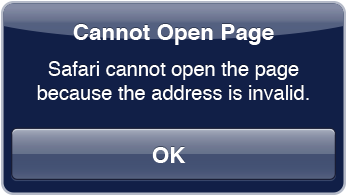
\includegraphics[width=0.35\textwidth]{img/customerror.png}
	\caption[Chybová hláška po otvorení custom URL schémy, pokiaľ aplikácia neexistuje]{
		Chybová hláška po otvorení custom URL schémy, pokiaľ aplikácia neexistuje \cite{customscheme}.\\
		Prevzaté z http://www.lukew.com/ff/entry.asp?1654}
	\label{fig: customerror}
\end{figure}

Lepším riešením je detekovanie, či si používateľ stiahol natívnu aplikáciu a odkaz na otvorenie v nej vytvoriť až potom, čo je overenie úspešné. Pokiaľ by nebolo, tak by sa mohlo zobraziť tlačítko na stiahnutie natívnej aplikácie, ktoré opäť musí byť prispôsobené platforme na ktorej na stránku prispôsobujeme, pokiaľ nechceme používateľa zahltitť všetkými platformami ktoré podporujeme.

Samotný proces detekcie či má používateľ nainštalovanú našu aplikáciu vôbec nie je triviálny, pretože na webe neexistuje žiadne dostupné API, ktoré by zahrňovalo všetky platformy. Apple síce vydal možnosť otvorenia aplikácie pomocou ,,Smart Banners'', ale až v iOS 6 a tak táto možnosť nie je úplne použiteľná.

\begin{figure}[H]
	\centering
	
\includegraphics[width=0.5\textwidth]{img/smartappbanner.png}
	\caption[Otvorenie natívnej aplikácie v iOS 6]{
		Otvorenie natívnej aplikácie v iOS 6 \cite{smartappbanner}.\\
		Prevzaté z http://developer.apple.com/}
	\label{fig: smartappbanner}
\end{figure}

Navyše ,,smart banner'' je priamo definovaný v html meta tagu aplikácie. Na stránke existuje len jeden ktorý volá url schému aplikácie a aj ten má prednastevený vzhľad v podobne okna v hornej časti obrazovky. Keby chceme vlastnú natívnu aplikáciu zavolať z viacerých častí webovej, prípadné volať viacero natívnych aplikácií, tak toto riešenie je nepostačujúce. Nemôže byť upravané vlastným potrebám.

Jediné možné riešenie je len v spolupráci s natívnou aplikáciou, aj tak sa však musí vyvolať otvorenie stránky v prehliadači, kde sa dá už do cookies alebo lokálneho úložiska programátorksy zapísať existencia aplikácie. Vytvorenie samotného ,,webView'' komponentu s webovou stránkou vrámci aplikácie a následné zatvorenie nestačí. Prehliadač má oddelené úložiská stránok pre rôzne typy prístupov ako sú s internetový prehliadač, aplikácia a v iOS aj pre otvorenie internetovaj stránky z plochy. Možnosť ako tento proces zamaskovať je skrytá v procese registrácie, keď po otvorení aplikácie a zaregistrovaní pošleme používateľovi e-mail s potvrdzujúcim odkazom, ktorý otvorí webovú stránku v prehliadači.


% subsubsection otvorenie_v_aplik_cii (end)

% subsection komponenty (end)

% section n_stroj_na_overenie (end)

\section{Overenie} % (fold)
\label{sec:overenie}

% section overenie (end)

\section{Záver} % (fold)
\label{sec:z_ver}

% section z_ver (end)